\documentclass[12pt]{article}
\usepackage[T1]{fontenc}
\usepackage[utf8]{inputenc}
\usepackage[english]{babel}
\babelprovide[main,import=pt-BR]{brazilian}
\usepackage{graphicx,booktabs,tabularx,amsmath,xurl}
\usepackage[hidelinks]{hyperref}
\usepackage{sbc-template}
\sloppy
\raggedbottom
\urlstyle{same}
\renewcommand{\topfraction}{0.9}
\renewcommand{\bottomfraction}{0.8}
\renewcommand{\textfraction}{0.1}
\renewcommand{\floatpagefraction}{0.8}
\graphicspath{{figuras/}}
\hypersetup{
 pdftitle={Integração de dados públicos de cobertura vacinal e sarampo},
 pdfauthor={Gabriel Eichelberger Fontaneli; João Villanova do Amaral; Rafaele Castagnara Alves},
 pdfsubject={Plataforma Streamlit, integração de dados e análise descritiva}}

\title{Integração de dados públicos de cobertura vacinal e sarampo:\\
uma plataforma interativa para o Rio Grande do Sul}
% Nomes abreviados apenas para manter a linha de autoria do modelo SBC.
\author{Gabriel E. Fontaneli\inst{1}, João Villanova do Amaral\inst{1}, Rafaele C. Alves\inst{1}}
\address{Instituto de Informática -- Universidade Federal do Rio Grande do Sul (UFRGS)\\
Caixa Postal 15.064 -- 91.501-970 -- Porto Alegre -- RS -- Brasil
\email{gefontaneli@inf.ufrgs.br, jvamaral@inf.ufrgs.br, rcalves@inf.ufrgs.br}}

\begin{document}
\maketitle

\begin{abstract}
This paper presents a working platform integrating 70 public files on MMR vaccination, measles and population in Brazil, covering 2015--2026 and detailing 497 municipalities in Rio Grande do Sul. Python and SQLite support data preparation and queries; Streamlit and Plotly provide six pages with filters and exports. Automated tests reproduce the original report's results. Analyses highlight second-dose coverage below target and sensitivity to annual aggregation methods. Partial periods, sparse events and unreconciled differences from official summaries limit interpretation. The contribution is a reproducible integration tool intended to support local health teams, without inferring causality.
\end{abstract}

\begin{resumo}
Este trabalho apresenta uma plataforma implementada que integra 70 arquivos públicos de vacinação, sarampo e população entre 2015 e 2026, detalhando 497 municípios gaúchos. Python e SQLite sustentam o tratamento e as consultas; Streamlit e Plotly oferecem seis páginas com filtros e exportação. Testes automatizados reproduzem os resultados do anteprojeto. As análises destacam cobertura da segunda dose abaixo da meta e sensibilidade ao método de agregação anual. Períodos parciais, eventos esparsos e divergências com balanços oficiais limitam a interpretação. A contribuição é uma ferramenta reprodutível de integração para apoiar equipes locais, sem inferência causal.
\end{resumo}

\section{Introdução}
A vacinação previne doenças, complicações e mortes, além de contribuir para reduzir a circulação de agentes infecciosos. No caso do sarampo, doença viral de elevada transmissibilidade, a Organização Mundial da Saúde (OMS) estima que a vacinação evitou aproximadamente 59 milhões de mortes entre 2000 e 2024 \cite{oms2026}. A vacina Tríplice Viral protege contra sarampo, caxumba e rubéola; seu monitoramento é relevante para a atenção primária e para a vigilância epidemiológica.

A proteção coletiva, também chamada de imunidade de rebanho, ocorre quando a presença de pessoas imunes dificulta a transmissão e beneficia indiretamente pessoas suscetíveis. Para o sarampo, a OMS recomenda alcançar e manter cobertura de pelo menos 95\% com duas doses em cada distrito \cite{omssarampo}. No Brasil, a meta de cobertura da Tríplice Viral adotada pelo Programa Nacional de Imunizações (PNI) é de 95\% \cite{manual2024}. Essa meta orienta o acompanhamento dos serviços: uma média estadual elevada não garante distribuição homogênea da proteção, e cobertura administrativa não equivale a uma medição direta da imunidade de toda a população.

Comparar Porto Alegre, o Rio Grande do Sul (RS) e o Brasil exige integrar vacinação, ocorrência da doença e população, disponíveis em arquivos com formatos, códigos, períodos e regras distintos. O problema computacional abordado é tornar essa integração rastreável e consultável, preservando as limitações de cada fonte.

O contexto de aplicação é o PET-Saúde: Informação e Saúde Digital, voltado à integração entre formação, serviços e comunidade \cite{petsaude}. A plataforma pretende apoiar preceptores e equipes das Unidades Básicas de Saúde (UBS), ainda sem avaliação em uso real. Integra cobertura da primeira (D1) e segunda dose (D2), aplicações mensais e casos de sarampo por \textbf{ano de início do exantema}, calculando incidência por 100 mil habitantes. O exantema é um dos sintomas, não um sinônimo do início de todos os sintomas.

Este artigo atualiza o anteprojeto para descrever a implementação em Python, SQLite e Streamlit/Plotly. A contribuição é a integração reprodutível para consulta territorial, sem estimar eficácia vacinal nem atribuir causalidade aos cruzamentos. As Seções 2 a 4 apresentam dados, ambiente e metodologia; a Seção 5, funcionalidades e resultados; a Seção 6, validação e pendências; e a Seção 7 conclui.

\section{Descrição da base de dados}
O acervo contém 70 arquivos nacionais, das 27 Unidades da Federação (UFs) e dos 497 municípios do RS. Somente o RS possui detalhamento municipal. A cobertura abrange 2015--2026; aplicações, numeradores e denominadores mensais estão disponíveis desde 2023. O processamento populacional utiliza 2015--2025 e replica 2025 para a incidência de 2026.

\begin{table}[!htbp]
\centering
\caption{Acervo utilizado e recortes disponíveis na versão atual.}
\label{tab:fontes}
\small
\begin{tabularx}{\textwidth}{@{}>{\raggedright\arraybackslash}p{3.1cm}rX@{}}
\toprule
Fonte e formato & Arquivos & Conteúdo e temporalidade \\
\midrule
TABNET/SI-PNI, CSV & 16 & Cobertura anual D1/D2, 2015--2022; não inclui doses absolutas nem população-alvo. \\
SEIDIGI/DEMAS, XLSX & 16 & Cobertura, numerador e população-alvo mensais, 2023--2026; em 2026, janeiro--agosto. \\
SEIDIGI/DEMAS, XLSX & 16 & Aplicações mensais D1/D2, todas as idades, 2023--2026; em 2026, janeiro--outubro. \\
SINAN/TABNET, CSV & 20 & Dois arquivos por ano de início do exantema e 18 cortes por ano de notificação; atualização informada até setembro/2026. \\
IBGE/Base dos Dados, CSV & 2 & População por UF e município, 1991--2025; 2026 utiliza o denominador de 2025. \\
\bottomrule
\end{tabularx}
\end{table}

Os arquivos de vacinação e de vigilância provêm dos sistemas divulgados pelo Ministério da Saúde \cite{tabnet,paineis}. A população tem origem no IBGE e foi obtida pela Base dos Dados \cite{basedados}. A aquisição ocorreu por exportação manual dos portais; o ETL lê o acervo local e não executa coleta automatizada. As planilhas de cobertura registram extração em 23/10/2026 e os CSVs do SINAN informam disponibilização no TABNET em setembro de 2026. Não há uma data de aquisição individual documentada para todo o acervo; a modificação local de um arquivo não é usada como equivalente à data de extração da fonte.

\subsection{Modelo relacional e dicionário resumido}
O modelo contém quatro entidades principais e três tabelas de apoio (Figura~\ref{fig:modelo}). A localidade possui identificador interno e código IBGE único: 00 para Brasil, dois dígitos para UFs e seis para municípios. Há unicidade nas combinações localidade--ano e localidade--ano--mês--dose.

\begin{figure}[!htbp]
\centering
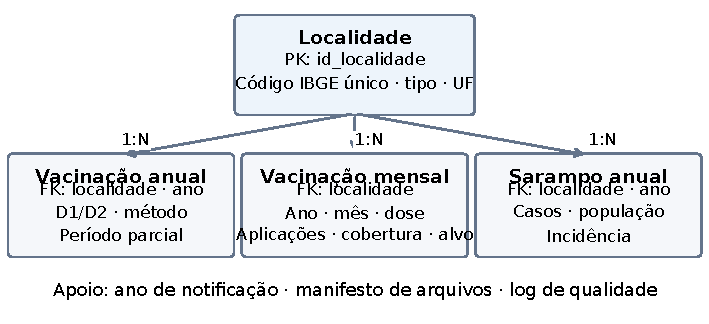
\includegraphics[width=\textwidth]{modelo_relacional.pdf}
\caption{Estrutura principal do banco. As setas representam relações 1:N de Localidade com cada tabela de fatos. As tabelas de apoio preservam outro critério de data e a rastreabilidade.}
\label{fig:modelo}
\end{figure}

\begin{table}[!htbp]
\centering
\caption{Dicionário resumido e volume carregado no SQLite.}
\label{tab:modelo}
\small
\begin{tabularx}{\textwidth}{@{}>{\raggedright\arraybackslash}p{3.6cm}rX@{}}
\toprule
Tabela & Linhas & Grão e principais informações \\
\midrule
LOCALIDADE & 525 & Um território: nome, código IBGE, tipo, UF e região. \\
VACINACAO\_\allowbreak ANUAL & 6.300 & Localidade--ano: D1/D2, métodos, numeradores, populações-alvo e período parcial. \\
VACINACAO\_\allowbreak MENSAL & 48.208 & Localidade--ano--mês--dose: aplicações, cobertura, numerador infantil e população-alvo. \\
NOTIFICACAO\_\allowbreak SARAMPO & 6.300 & Localidade--ano de exantema: casos, população, incidência e sinalizações. \\
NOTIFICACAO\_\allowbreak ANO\_\allowbreak NOTIF & 157 & Localidade--ano de notificação: comparação entre critérios de data. \\
FONTE\_\allowbreak ARQUIVO & 70 & Arquivo: origem, conteúdo, linhas, datas e hash SHA-256. \\
LOG\_\allowbreak QUALIDADE & 28 & Ocorrências de limpeza e integração: descrição e quantidade. \\
\bottomrule
\end{tabularx}
\end{table}

O núcleo soma 61.333 registros, e o banco completo contém 61.588 linhas em sete tabelas, ocupando aproximadamente 4,3 MB. Os 48.208 registros mensais correspondem a 524 territórios, duas doses e 46 meses disponíveis; não há uma linha mensal nacional própria. As populações-alvo de D1 e D2 são armazenadas separadamente porque diferem nas planilhas.

A separação entre cadastro e observações evita repetir atributos descritivos. Incidência, coberturas e indicadores de meta são materializados; não se afirma terceira forma normal estrita para todo o esquema físico. A consistência depende do ETL; as consultas classificam a cobertura conforme o método selecionado.

\section{Ambiente de desenvolvimento}
A aplicação utiliza Python no tratamento, SQLite no armazenamento e Streamlit/Plotly na interface. O SQLite dispensa servidor dedicado e favorece a simplicidade operacional \cite{sqlite}; não foi realizado estudo de desempenho sob múltiplos usuários ou grandes cargas.

O ambiente verificado foi Python 3.14.10, SQLite 3.54.0, pandas 3.1.1, NumPy 2.5.5, openpyxl 3.1.5, XlsxWriter 3.3.1, Plotly 7.1.0, Streamlit 1.67.0, SciPy 1.18.1 e pytest 9.2.0. Os arquivos de requisitos registram versões diretas e transitivas. Não se presume configuração de hardware dos autores. As figuras do artigo foram geradas separadamente com Matplotlib 3.11.2, a partir do mesmo banco; essa biblioteca não é dependência da interface.

O projeto separa extratores, carga, consultas, estatística e interface, que abre o banco somente para leitura. O cache considera caminho, identificação, modificação e tamanho do arquivo, renovando consultas e conexão quando o ETL recria o banco. Seus parâmetros de versão participam da chave do cache, conforme a documentação \cite{streamlitcache}.

\section{Metodologia}
O estudo utiliza dados agregados, sem identificação individual. O fluxo compreende leitura, padronização, integração territorial e temporal, carga, consultas e apresentação. O recorte desta revisão é 22/11/2026.

\subsection{Tratamento e controle de qualidade}
O tratamento interpreta latin1, ponto e vírgula e vírgula decimal nos CSVs do TABNET. Nas planilhas, reorganiza cabeçalhos de três linhas e converte proporções em porcentagem. O código municipal do IBGE, com sete dígitos, é compatibilizado com os seis das demais fontes e verificado contra o cadastro territorial.

As matrizes de sarampo são transformadas em registros localidade--ano de 2015--2026. Anos anteriores e exantema sem ano informado são registrados no log, sem redistribuição. Traços e ausência municipal são interpretados como zero, sem eliminar a possibilidade de subnotificação. O total nacional inclui UF ignorada/exterior: 21.797 registros em 2019, contra 21.781 nas 27 UFs.

O ETL mantém cobertura ausente como nula: quatro registros municipais em 2015, 2016, 2021 e 2022. Descarta uma linha populacional sem UF e 535 linhas municipais incompletas. Confere e deduplica totais do RS repetidos nos arquivos, sem divergências nos campos comparados. O hash SHA-256 identifica cada arquivo utilizado.

\subsection{Definição dos indicadores}
Para a localidade $i$ no ano $t$, a incidência apresentada é
\begin{equation}
 I_{it}=\frac{C_{it}}{P_{it}}\times 100.000,
\end{equation}
em que $C_{it}$ representa registros de sarampo por ano de início do exantema e $P_{it}$ é a população residente. O banco armazena quatro casas decimais; as tabelas da interface normalmente mostram duas. Assim, um valor exibido como 0,00 não demonstra ausência de casos. Para comparar grupos territoriais, a taxa usa a soma dos casos dividida pela soma das populações, e não a média simples das incidências municipais.

Entre 2015 e 2022, a cobertura anual é a taxa fornecida pelo TABNET. Para 2023--2026, a aplicação oferece dois métodos. Se $r_m$ é a proporção mensal informada, $n_m$ o numerador da cobertura, $p_m$ a população-alvo e $M$ o número de meses disponíveis, os cálculos implementados são
\begin{equation}
 CV_{\text{média}}=\frac{1}{M}\sum_{m=1}^{M}100r_m,
 \qquad
 CV_{\text{razão}}=100\frac{\sum_m n_m}{\sum_m p_m}.
\end{equation}
A média simples é o padrão da interface e reproduz a tabela do anteprojeto; a razão das somas é uma alternativa de sensibilidade. Essa reprodução não comprova equivalência à cobertura anual oficial. Além disso, a Nota Técnica nº 90/2025 descreve mudança, a partir de 2024, para o indivíduo vacinado como unidade do numerador \cite{nota90}. A comparabilidade entre fontes e períodos exige validar as regras de extração e agregação, não apenas aplicar a mesma fórmula.

Há 3.144 registros mensais com população-alvo zero; a fonte utiliza a sentinela $10^{-6}$ na proporção, convertida em 0,0001\%. A implementação atual incorpora essa sentinela na média mensal e mantém os numeradores na razão das somas. Ambos os comportamentos são aqui documentados como limitações ainda pendentes de validação. Não se substituem silenciosamente os valores para produzir este artigo, nem se apresenta a alternativa como uma correção já homologada.

Aplicações em todas as idades diferem dos numeradores da cobertura infantil: a D1 de Porto Alegre em 2025 soma 19.761 aplicações e 11.713 no numerador da cobertura. D1 menos D2 tampouco mede abandono individual: populações-alvo e coortes podem diferir, sem seguimento das mesmas pessoas.

\subsection{Períodos parciais e exploração estatística}
Em 2026, cobertura abrange janeiro--agosto, aplicações janeiro--outubro e vigilância apresenta atualização em setembro. Outubro pode estar incompleto; os casos disponíveis são anuais e não permitem comparação mensal equivalente. Esses valores não devem ser comparados diretamente a totais de anos completos. A população de 2025 é reutilizada porque é a última disponível \emph{no acervo}; não se afirma inexistência de estimativas mais recentes fora dele. Se a população real de 2026 for maior, a incidência calculada será superestimada, e vice-versa.

A interface permite comparar cobertura e incidência no mesmo ano ou com defasagem de um ou dois anos, agrupando localidades abaixo de 95\% e com 95\% ou mais. O módulo secundário calcula Spearman, p-valor assintótico e intervalo aproximado de Fisher. Esses resultados são exploratórios: a documentação do SciPy alerta para a precisão do p-valor em amostras menores e sugere considerar testes de permutação \cite{scipy}. Empates por ausência de casos, dependência espacial, filtros e diferentes composições etárias limitam a inferência. A análise restrita a localidades com casos altera a população estudada e não substitui a análise de todas as localidades elegíveis.

\section{Funcionalidades e resultados}
\subsection{Da proposta à interface implementada}
As quatro consultas básicas e duas operações avançadas do anteprojeto foram implementadas em funções reutilizáveis, com filtros parametrizados. A Tabela~\ref{tab:paginas} relaciona essa proposta às seis páginas atuais. A comparação por UF usa o ano escolhido; a série histórica aceita diferentes localidades. As particularidades das fontes são acessíveis em avisos e 2026 recebe sinalização visual. As tabelas oferecem CSV e Excel; os gráficos permitem PNG pelo controle do Plotly e download em HTML interativo.

\begin{table}[!htbp]
\centering
\caption{Funcionalidades disponíveis na navegação oficial.}
\label{tab:paginas}
\small
\begin{tabularx}{\textwidth}{@{}p{3.4cm}X@{}}
\toprule
Página & Recursos implementados e relação com o anteprojeto \\
\midrule
Visão geral & Indicadores do ano escolhido para Brasil, RS e Porto Alegre; evolução D1/D2 e casos; leitura rápida. \\
Cobertura vacinal & Série histórica (CB1), D1/D2 por UF (CB2), municípios na meta e tabela por situação, nome e faixa de cobertura (CB4). \\
Casos e incidência & Ranking municipal, estadual ou nacional (CB3); seleção de ano ou intervalo, população mínima, casos mínimos e ordenação. \\
Cobertura $\times$ sarampo & Junção localidade--ano (CA1); comparação por meta, defasagem, dispersão, Spearman e contexto epidemiológico com fontes. \\
Ficha do município & Cobertura, casos, incidência e séries anuais; aplicações mensais com uma linha por ano e painéis D1/D2 (CA2); Excel com duas abas. \\
Dados e metodologia & Manifesto de fontes, modelo, dicionário, log, limitações, versões e consultas SQL em texto expansível. \\
\bottomrule
\end{tabularx}
\end{table}

A consulta mensal é utilizada na ficha municipal; não há página independente de doses mensais ou versões experimentais na navegação oficial. Os filtros não ampliam o escopo geográfico do acervo.

\subsection{Cobertura e ocorrência de sarampo}
A Figura~\ref{fig:cobertura} reorganiza os dados da série exibida pelo dashboard em dois painéis para facilitar a leitura no artigo. Utiliza o método padrão e mantém a distinção entre fonte anual e agregação mensal. A D2 permanece abaixo de 95\% em todos os 11 anos completos, de 2015 a 2025, para Brasil, RS e Porto Alegre. A recuperação após 2021 não elimina a distância da meta. Os pontos de 2026 também ficam abaixo dela, mas representam recorte parcial.

\begin{figure}[!htbp]
\centering
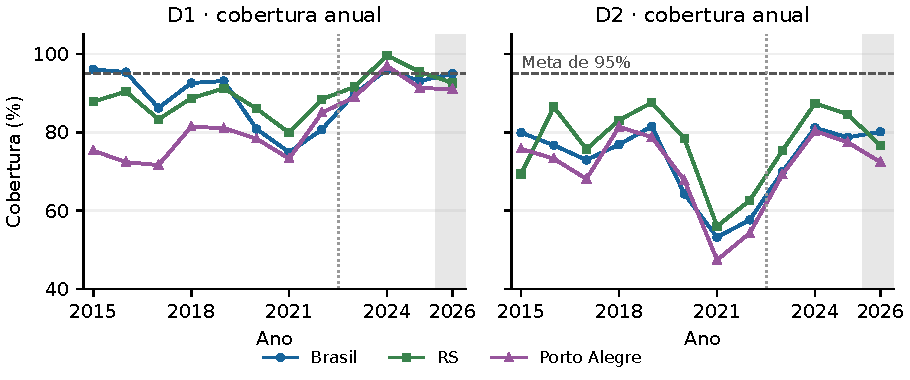
\includegraphics[width=\textwidth]{cobertura_historica.pdf}
\caption{Cobertura D1/D2 no banco do projeto. De 2023 em diante, média simples mensal; a linha vertical marca a mudança de fonte. A faixa cinza identifica 2026 parcial. Fonte: elaboração própria com dados do SQLite.}
\label{fig:cobertura}
\end{figure}

Em 2025, último ano completo, D1/D2 são 93,14\%/78,72\% no Brasil, 95,44\%/84,62\% no RS e 91,35\%/77,47\% em Porto Alegre. A capital tem um caso e incidência de 0,0720 por 100 mil. As 36 linhas históricas permanecem disponíveis nos dados complementares.

O banco registra 21.797 casos nacionais em 2019 e 39.136 entre 2018 e 2020. Esses números descrevem o acervo integrado e não são automaticamente intercambiáveis com balanços revisados do Ministério da Saúde. Por exemplo, o banco contém quatro registros em 2023 e 42 em 2025, enquanto as publicações consultadas informam zero e 38 casos confirmados, respectivamente \cite{balanco2026,situacao}. A causa dessas diferenças não foi reconciliada; o painel apresenta os totais separadamente. Essa distinção impede que um registro do arquivo seja usado, isoladamente, para afirmar a ocorrência de surto confirmado.

O Brasil recuperou em 2024 a certificação de eliminação da circulação endêmica do sarampo \cite{situacao}. Isso não significa erradicação global nem ausência permanente de casos importados. A série integrada não demonstra, isoladamente, causas de surtos.

\subsection{Por que combinar casos e incidência?}
No RS, 23 municípios possuem pelo menos um registro de sarampo ao longo de 2015--2026, totalizando 189 casos na base. Porto Alegre soma 68, mas não lidera necessariamente as taxas. A Figura~\ref{fig:incidencia} contrasta seis exemplos de 2019, sem pretender constituir um ranking completo. Gravataí apresenta 35 casos e incidência de 12,43 por 100 mil; Porto Alegre, 22 casos e 1,48; Cachoeirinha, 20 e 15,35. Em Carlos Gomes, um único caso em 1.377 habitantes produz 72,62 por 100 mil.

\begin{figure}[!htbp]
\centering
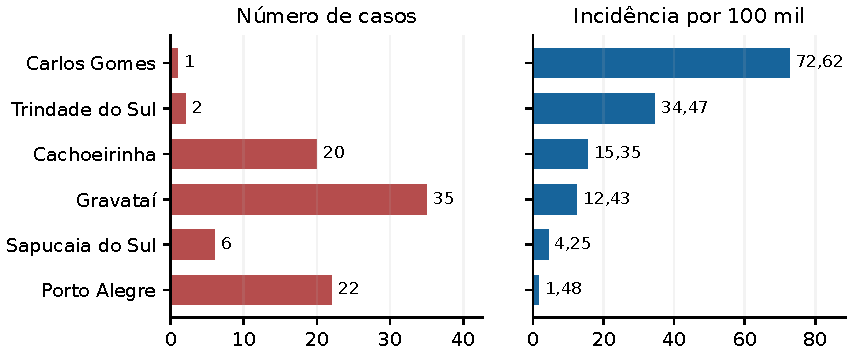
\includegraphics[width=\textwidth]{casos_incidencia_2019.pdf}
\caption{Exemplos municipais de 2019: mesmos territórios, número absoluto e incidência em painéis separados. Taxas elevadas podem decorrer de denominadores pequenos. Fonte: elaboração própria com dados do projeto.}
\label{fig:incidencia}
\end{figure}

No ranking acumulado, a tela soma taxas anuais e filtra anos sem casos antes de agregar. A população exibida pode, portanto, corresponder ao último ano com casos, não ao último selecionado. A medida exige revisão; os exemplos desta seção utilizam um único ano, com casos e incidência apresentados conjuntamente.

\subsection{Aplicações mensais na ficha do município}
A Figura~\ref{fig:mensal} apresenta as aplicações da ficha de Porto Alegre, separadas por dose e ano. A linha de 2026 termina em outubro; novembro e dezembro são ausentes, não zeros. Os picos permitem levantar hipóteses sobre campanhas, demanda e registro, mas os arquivos não identificam suas causas.

\begin{figure}[!htbp]
\centering
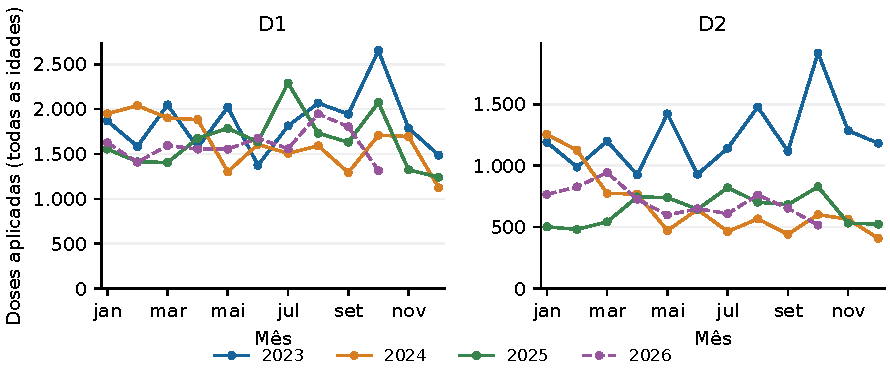
\includegraphics[width=\textwidth]{doses_mensais_poa.pdf}
\caption{Aplicações mensais da Tríplice Viral em Porto Alegre, 2023--2026, por dose e ano. A linha tracejada representa 2026 parcial. Não se trata da contagem exclusiva da população-alvo da cobertura. Fonte: elaboração própria.}
\label{fig:mensal}
\end{figure}

\subsection{Sensibilidade da cobertura anual e relação exploratória}
Em 2025, 334 municípios atingem 95\% de D1 e 260 atingem 95\% de D2 pelo método padrão. Na razão das somas, são 340 e 236. A Tabela~\ref{tab:sensibilidade} mostra também quantos municípios \emph{mudam de grupo}, independentemente da direção. Esse número é maior que a diferença líquida entre os totais porque há mudanças nos dois sentidos.

\begin{table}[!htbp]
\centering
\caption{Sensibilidade à agregação anual nos 497 municípios do RS.}
\label{tab:sensibilidade}
\small
\begin{tabular}{@{}crrrrrr@{}}
\toprule
 & \multicolumn{2}{c}{D1: na meta} & \multicolumn{2}{c}{D2: na meta} & \multicolumn{2}{c}{Mudam de grupo} \\
Ano & Média & Razão & Média & Razão & D1 & D2 \\
\midrule
2023 & 305 & 261 & 217 & 146 & 116 & 127 \\
2024 & 354 & 340 & 278 & 256 & 132 & 132 \\
2025 & 334 & 340 & 260 & 236 & 134 & 138 \\
2026* & 266 & 241 & 182 & 153 & 105 & 117 \\
\bottomrule
\end{tabular}
\par\smallskip
\footnotesize *Janeiro--agosto. Os métodos são alternativas implementadas; sua equivalência à cobertura anual oficial ainda requer validação.
\end{table}

Em Água Santa, por exemplo, D1/D2 de 2025 são 139,66\%/98,91\% pela média e 76,92\%/69,23\% pela razão. A mudança de classificação em 138 municípios para D2 representa 27,8\% do RS. Resultados municipais e classificações frente à meta precisam, portanto, ser acompanhados do método, e não interpretados como independentes dessa escolha. Cobertura acima de 100\% é preservada como informada; não constitui prova de proteção integral de residentes.

A relação exploratória acrescenta uma leitura complementar. Para D2 em 2019, mantendo os filtros disponíveis no painel e população mínima de 5.000 habitantes, são elegíveis 266 municípios: 156 abaixo de 95\% e 110 na meta. Os grupos somam 102 e dois casos, respectivamente; suas incidências agregadas são 1,218 e 0,087 por 100 mil. Um caso do RS fica fora desse recorte populacional. O coeficiente de Spearman entre cobertura e incidência é aproximadamente $-0,158$ nesse conjunto.

Esse resultado não demonstra que a cobertura do ano causou ou preveniu os eventos. Há somente 31 pares município--ano com casos entre 3.976 possíveis em 2018--2025, além de diferenças de idade, circulação regional e importação. Nas UFs, por exemplo, todas ficam abaixo de 95\% em D2 em 2019, impossibilitando comparar dois grupos nesse recorte. A interface informa grupos vazios e ausência de variação; p-valores e intervalos permanecem em detalhes, sem fundamentar conclusões causais neste artigo.

\section{Validação, atendimento às avaliações e próximos passos}
A verificação de 22/11/2026 aprovou os 82 testes de extração, integração, consultas, estatística, páginas e cache. Foram reproduzidas as 36 linhas históricas do anteprojeto para Brasil, RS e Porto Alegre. Os testes abrangem cobertura ausente, grupos vazios, anos sem casos, filtros e substituição do SQLite. Demonstram consistência com as regras implementadas, não validação epidemiológica externa ou usabilidade.

Os resultados foram recalculados do banco em modo somente leitura. O material complementar inclui gerador das figuras, dados e hash do banco. São gráficos autorais, sem representar uma nova interface. O texto utiliza o estilo SBC fornecido; equações, tabelas e gráficos substituem as listagens SQL/Python.

As avaliações do JEMS orientaram avisos, exportações, filtros, documentação de versões e datas, comparação mensal por ano e um modelo legível. Foram corrigidos o título e a terminologia epidemiológica.

Expandir municípios para outras UFs exige novos arquivos. Estimar doses de 2015--2022 exige populações-alvo ausentes; a população total não pode substituí-las. A análise estatística foi incorporada como exploração, sem estimar efeitos individuais.

ETL, banco, consultas, interface e testes estão concluídos. Permanecem pendentes a validação epidemiológica, a reconciliação dos casos, a correção do ranking acumulado, a avaliação com preceptores e a publicação em nuvem. O efeito das revisões populacionais sobre cobertura infantil exige examinar a população-alvo específica, além do denominador IBGE da incidência. A avaliação poderá registrar conclusão, dificuldades e tempo em tarefas de localizar municípios abaixo da meta, comparar séries, identificar meses de menor aplicação e exportar fichas. Ainda não foram coletados resultados de uso, satisfação ou impacto na rotina das UBS.

\section{Considerações finais}
A plataforma transforma 70 arquivos heterogêneos em um banco relacional consultável e uma interface com seis páginas oficiais, possibilitando examinar cobertura da Tríplice Viral, casos de sarampo, incidência e aplicações mensais. A implementação incorpora filtros, exportações, rastreabilidade e testes, avançando além do planejamento descrito no anteprojeto. Os exemplos evidenciam a distância da D2 em relação à meta, a diferença entre volume absoluto e taxas e a sensibilidade municipal à agregação anual.

A contribuição é organizar dados verificáveis para análises territoriais no PET-Saúde Digital. Permanecem essenciais a validação dos indicadores e a avaliação com usuários. A interpretação deve distinguir cobertura administrativa de imunidade populacional, dados locais de balanços oficiais e associação ecológica de causalidade, respeitando o que o acervo e a avaliação atual permitem concluir.

\bibliographystyle{sbc}
\bibliography{referencias}
\end{document}
